\documentclass[12pt,a4paper]{article}
\usepackage[tikzit]{mrw}

\usepackage[hidelinks]{hyperref}
\usepackage{xltabular}
\usepackage{booktabs}
\usepackage{pdfpages}

\pagestyle{fancy}
\fancyhead[L]{Part II Project Proposal}
\fancyhead[R]{Martin Walls}
\fancyfoot[C]{\thepage\ / \pageref{LastPage}}
\fancypagestyle{firstpage}{
  \fancyhead{}
  \renewcommand{\headrulewidth}{0em}
  \fancyfoot[C]{\thepage\ / \pageref{LastPage}}
}

\title{Part II Project Proposal: C to WebAssembly Compiler}
\author{Martin Walls}
\date{October 2022}

\begin{document}

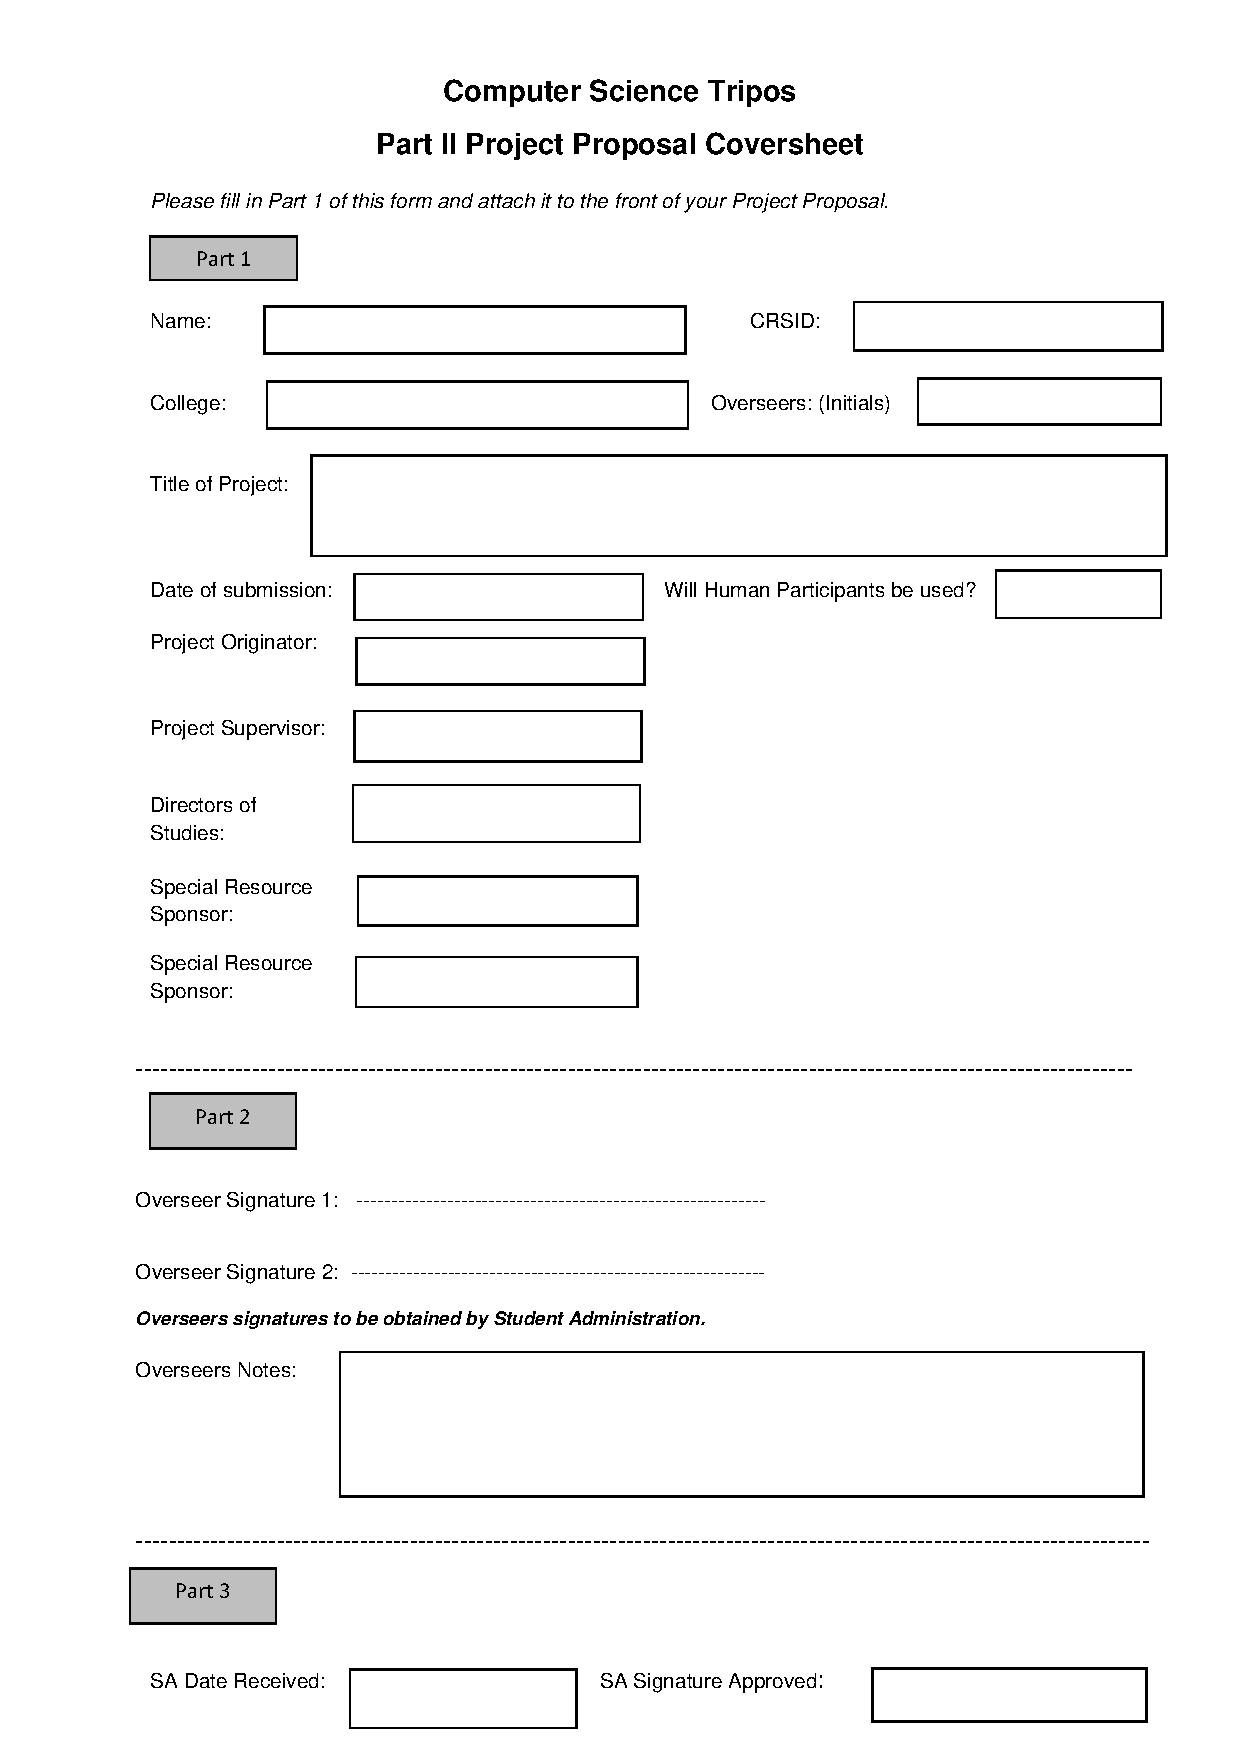
\includepdf[
  picturecommand={
    \put(145,682){Martin Walls}
    \put(430,684){mrw64}
    \put(145,646){Churchill}
    \put(455,648){SH, NK}
    \put(165, 605){C to WebAssembly Compiler}
    \put(185, 553){14 October 2022}
    \put(490, 555){No}
    \put(185, 522){Timothy M. Jones}
    \put(185, 485){Timothy M. Jones}
    \put(185, 448){Dr John K. Fawcett}
  }
]{12-proposal-cover-sheet}

\setcounter{page}{1}

\maketitle
\thispagestyle{firstpage}

\section*{Overview}

With the web playing an ever-increasing role in how we interact with computers, applications are often expected to run in a web browser in the same way as a traditional native application. Web\-Assembly is a binary code format that runs in a stack-based virtual machine, supported by all major browsers. It aims to bring near-native performance to web applications, with applications for situations where JavaScript isn't performant enough, and for running programs originally written in languages other than JavaScript in a web browser.

I plan to implement a compiler from the C language to WebAssembly.
C is a good candidate for this project because it is quite a low-level language, so I can focus on compiler optimisations rather than just implementing language features to make it work. Because C has manual memory management, I won't have to implement a garbage collector or other automatic memory management features.
Initially I will provide support for the stack only, and if time allows I will implement \texttt{malloc} and \texttt{free} functionality to provide heap memory management.

I will compile a subset of the C language, to allow simple C programs to be run in a web browser. A minimal set of features to support will include arithmetic, control flow, variables, and functions (including recursion).
I won't initially implement linking, so the compiler will only handle single-file programs. This includes not linking the C standard library, so I will provide simple implementations of some of the standard library myself, as necessary to provide common functionality such as \texttt{printf}.

I will use a lexer and parser generator to do the initial source code transformation into an abstract syntax tree.
I will focus this project on transforming the abstract syntax tree into an intermediate representation---where optimisations can be done---and then generating the target WebAssembly code.

I plan to write the compiler in Rust, which is memory safe and performant, and has lexer/parser generators I can use.

To test and evaluate the compiler, I will write small benchmark programs that individually test each of the features and optimisations I add. For example, I will use the Fibonacci program to test recursion.
I will also test it with Conway's Game of Life, as an example of a larger program, to test and evaluate the functionality of the compiler as a whole.


I will use a three-address code style of intermediate representation, because this lends itself to perform optimisations more easily. For example it's easier to see the control flow in three-address code compared to a stack-based representation.
To transform from abstract syntax tree to the intermediate representation, this will involve traversing the abstract syntax tree recursively, and applying a transformation depending on the type of node to three-address code.



To transform from the intermediate representation to WebAssembly, I will need to convert the three-address code representation into a stack-based format, since WebAssembly is stack-based. This stack-based format will have a direct correspondence to WebAssembly instructions, so the final step of the compiler will be writing out the list of program instructions to a WebAssembly binary file.

C allows unstructured control flow (e.g.\ \texttt{goto}), whereas WebAssembly only supports structured control flow. Therefore I will need a step in the compiler to transform unstructured to structured control flow. One algorithm to do this is the Relooper algorithm, which was originally implemented as part of Emscripten, a LLVM to JavaScript compiler\footnote{\url{https://github.com/emscripten-core/emscripten/blob/main/docs/paper.pdf}}.

\subsection*{Compiler pipeline overview}

\tikzfig{11-overview-flowchart}



\section*{Starting point}

I don't have any experience in writing compilers beyond the Part IB Compiler Construction course. I haven't previously used any lexer or parser generator libraries.
I've briefly looked at Rust over the summer, but haven't written anything other than simple programs in it.

I have briefly looked up the instruction set for WebAssembly and have written a single-function program that does basic arithmetic, in WebAssembly text format. I used \texttt{wat2wasm} to convert this to a WebAssembly binary and ran the function using JavaScript.

I have briefly researched lexer and parser generators to see what's out there and to help decide on which language to write my compiler in, but I haven't used them before.

\section*{Success criteria}

The project will be a success if:

\begin{itemize}
\item The program generates an abstract syntax tree from C source code.
\item The program transforms the abstract syntax tree into an intermediate representation.
\item The program uses the Relooper algorithm to transform unstructured to structured control flow.
\item The program generates WebAssembly binary code from the intermediate representation.
\item The compiler generates binary code that produces the same output as the source program.
\end{itemize}


\section*{Optimisations}

First I will implement some simple optimisations, before adding some more complicated ones.

One of the simple optimisations I will implement is peephole optimisation, which is where we look at short sections of code and match them against patterns we know can be optimised, then replacing them with the optimised version.
For example, redundant operations can be removed, such as writing to the same variable twice in a row (ignoring the first value written), or a stack push followed immediately by a pop.
Null operations (operations that have no effect, such as adding zero) can also be removed.

Constant folding is another quite simple optimisation that performs some arithmetic at compile time already, if possible. For example, the statement \texttt{x = 3 + 4} can be replaced by \texttt{x = 7} at compile time; there is no need for the addition operation to be done at runtime.

These optimisations will be run in several passes, because doing one optimisation may then allow another optimisation to be done that wasn't previously available. The optimisation passes will run until no further changes are made.

The stack-based peephole optimisations (such as removing pushes directly followed by a pop) will be done once the three-address code representation has been transformed into the stack-based format in the final stage.

A more complicated optimisation to add will be tail-call optimisation, which removes unnecessary stack frames when a function call is the last statement of a function.

Other harder optimisations are left as extensions to the project.

\section*{Extensions}

Extensions to this project will be further optimisations. These optimisations are more complicated and will involve more analysis of the code.

One optimisation would be dead-code elimination, which looks through the code for any variables that are written to but never read. Code that writes to these variables is removed, saving processing power and space.

Another optimisation would be unreachable-code elimination, where we perform analysis to find blocks of code that can never be executed, and removing them. This will involve control flow analysis to determine the possible routes the program can take.


\section*{Evaluation}

To test and evaluate the compiler, I will use it to compile a variety of different programs. Some of these will be small programs I will write to specifically test the features and optimisations of the compiler individually. I will also write a larger test program to evaluate the compiler as a whole.

In addition, I will use some pre-existing benchmark programs to give a wider range of tests. For example, cBench is a set of programs for benchmarking optimisations, which I could choose appropriate programs from. The source for cBench is no longer available online, but my supervisor is able to give me a copy of them.

For each of these, I will verify that the generated WebAssembly code produces the same output as the source program when run.

To evaluate the impact of the optimisations, I will run the compiler once with optimisations enabled and once with them disabled, on the same set of programs. I will then benchmark the performance of the output program to identify the impact of the optimisations on the program's running time, and I will also compare the size of the two programs to assess the impact on storage space.

\section*{Work Plan}

\newcounter{workpackages}
\newcommand\workpackagenumber{\stepcounter{workpackages}\arabic{workpackages}}

\begin{xltabular}{\textwidth}{l>{\bfseries}lX}
\toprule
\workpackagenumber & 14th - 28th Oct &
Preparatory research, set up project environment, including toolchain for running compiled WebAssembly. I will research the WebAssembly instruction set.

I will also write test C programs for Fibonacci and Conway's Game of Life. To help with my WebAssembly research, I will implement the same Fibonacci program in WebAssembly by hand. \\
\addlinespace
& & \itshape\textbf{Milestone deliverable:} I will write a short LaTeX document explaining the WebAssembly instruction set, from the research I do.

C programs of Fibonacci and Conway's Game of Life, and a WebAssembly implementation of Fibonacci. \\
\midrule
\workpackagenumber & 28th Oct - 11th Nov &
Lexer and parser generator implementation.

This will involve writing the inputs to the lexer and parser generators to describe the grammar of the source code and the different types of tokens. \\
\addlinespace
& & \itshape\textbf{Milestone deliverable}: Lexer and parser generator inputs. The compiler will be able to generate an abstract syntax tree (AST) representation from a source program. \\
\midrule
\workpackagenumber & 11th - 25th Nov &
Implementation of transforming the AST into the intermediate representation.
This will require defining the intermediate code to generate for each type of node in the AST. \\
\addlinespace
& & \itshape\textbf{Milestone deliverable}: The compiler will be able to generate an intermediate representation version from a source program. \\
\midrule
\workpackagenumber & 25th Nov - 9th Dec &
Researching and implementing the Relooper algorithm. \\
\addlinespace
& & \itshape \textbf{Milestone deliverable}: The compiler will be able to transform unstructured control flow into structured control flow using the Relooper algorithm. I will also write a short LaTeX document describing the algorithm. \\
\midrule
\workpackagenumber & 9th - 23rd Dec &
Implementation of target code generation from intermediate representation.

For each type of instruction in the intermediate representation, I will need to define the transformation that generates WebAssembly from it. \\
\addlinespace
& & \itshape\textbf{Milestone deliverable}: The compiler will be able to generate target code for a source program. The generated WebAssembly will be able to be run in a web browser. \\
\midrule
& & \itshape Two weeks off over Christmas \\
\midrule
\workpackagenumber & 6th - 20th Jan &
\textit{\small(I'll be more busy during the first week of this with some extracurricular events before term.)}

Slack time to finish main implementation if necessary. Implement some peephole optimisations (how many I do here depends on how much of the slack time I need). \\
\addlinespace
& & \itshape \textbf{Milestone deliverable}: The basic compiler pipeline will be complete. Some peephole optimisations will be implemented. \\
\midrule
\workpackagenumber & 20th Jan - 3rd Feb &
Write progress report.

Continue implementing optimisations, in particular implementing tail-call optimisation. \\
\addlinespace
& & \itshape\textbf{Milestone deliverable}: Completed progress report. (Deadline 03/02) \\
\midrule
\workpackagenumber & 3rd - 17th Feb &
\textit{\small(I'll be more busy here with extra-curricular events.)}

Slack time to finish main optimisations if necessary. If time allows, work on extension optimisations. \\
\addlinespace
& & \itshape\textbf{Milestone deliverable}: The compiler will be able to generate target code with optimisations applied. Evidence to show the impact of the optimisations. \\
\midrule
\workpackagenumber & 17th Feb - 3rd Mar &
Evaluate the compiled WebAssembly using a variety of programs (as described above), including correctness and impact of optimisations. Write these evaluations into a draft evaluation chapter. \\
\addlinespace
& & \itshape\textbf{Milestone deliverable}: Draft evaluation chapter. \\
\midrule
\workpackagenumber & 3rd - 17th Mar &
Write introduction and preparation chapters. \\
\addlinespace
& & \itshape\textbf{Milestone deliverable}: Introduction and preparation chapters. \\
\midrule
\workpackagenumber & 17th - 31st Mar &
Write implementation chapter. \\
\addlinespace
& & \itshape\textbf{Milestone deliverable}: Implementation chapter. \\
\midrule
\workpackagenumber & 31st Mar - 14th Apr &
Write conclusions chapter and finish evaluations chapter. \\
\addlinespace
& & \itshape\textbf{Milestone deliverable}: Evaluations and conclusions chapter. First draft of complete dissertation. \\
\midrule
\workpackagenumber & 14th - 28th Apr &
Adjust dissertation based on feedback. \\
\addlinespace
& & \itshape\textbf{Milestone deliverable}: Finished dissertation. \\
\midrule
\workpackagenumber & 28th Apr - 12 May &
Slack time in two weeks up to formal deadline, to make any final changes. \\
\addlinespace
& & \itshape\textbf{Milestone deliverable}: Final dissertation submitted. (Deadline 12/05) \\
\bottomrule
\end{xltabular}


\section*{Resource declaration}

I will primarily use my own laptop for development. I accept full responsibility for this machine and I have made contingency plans to protect myself against hardware and/or software failure.

My laptop specifications are:
\begin{itemize}
\item Lenovo IdeaPad S540
\item CPU: AMD Ryzen 7 3750H
\item 8GB RAM
\item 2TB SSD
\item OS: Fedora 35
\end{itemize}

I will use Git for version control and will regularly push to an online Git repository on GitHub. I will clone this repository to the MCS and regularly update the clone, so that if my machine fails I can immediately continue work on the MCS.

\end{document}
